\newpage
\section{Zahlensysteme}

\subsection{Dezimal zu base-n umrechnen}
\begin{figure}[h!]
	\centering
	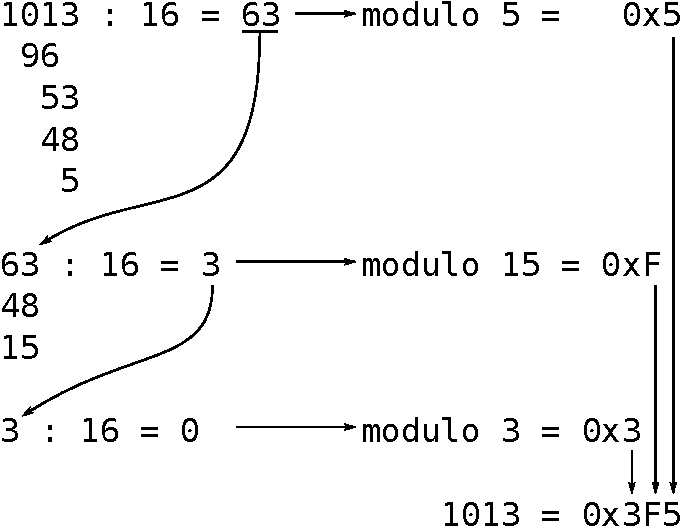
\includegraphics[scale=0.5]{../fig/dechex.pdf}
	\caption{Beispielrechnung Dezimal zu Hexadezimal}
\end{figure}

\subsection{signed zu unsigned unrechnen}
\begin{figure}[h!]
	\centering
	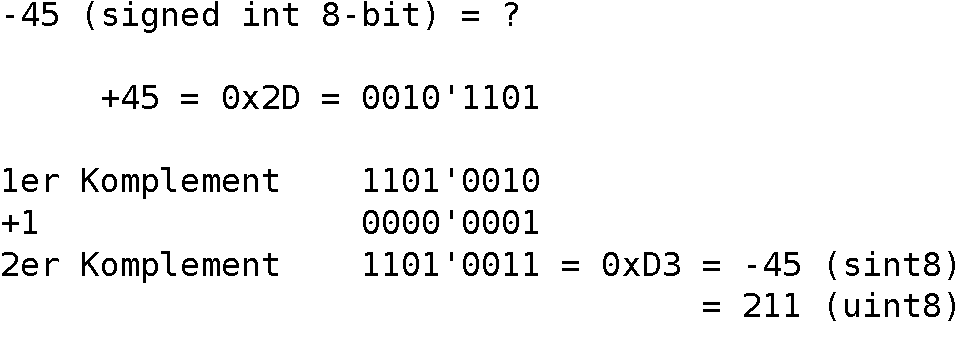
\includegraphics[scale=0.5]{../fig/signed.pdf}
	\caption{Beispielrechnung negative signed 8-Bit Zahl}
\end{figure}

\subsection{Endian}
\begin{figure}[h!]
	\centering
	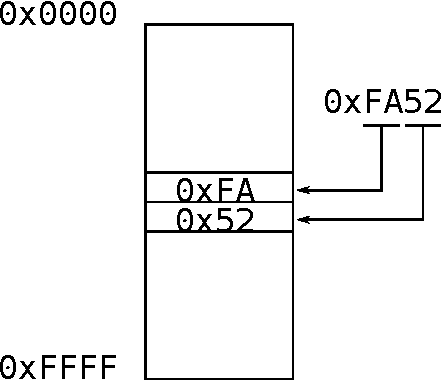
\includegraphics[scale=0.5]{../fig/endian.pdf}
	\caption{Eine 16-Bit Zahl in 8-Bit Speicher ablegen mit Big-Endian}
\end{figure}


